\chapter{METODOLOGI}

% Ubah konten-konten berikut sesuai dengan isi dari metodologi

\section{Bahan dan peralatan yang digunakan}

Peralatan yang digunakan untuk penelitian ini antara lain:

\begin{enumerate}
  \item \textbf{GraspNet}, digunakan sebagai \emph{framework} robot lengan untuk
  melakukan tugas berupa \emph{autonomous grasping}. GraspNet sendiri adalah sebuah \emph{framework}
  berbasis \emph{deep learning} yang dirancang untuk melakukan prediksi \emph{pose grasping} secara akurat bagi lengan robot.
  \item \textbf{ROS}, yang mana merupakan sebuah \emph{framework}
  \emph{open-source} yang menyediakan kumpulan \emph{software}, \emph{library}, dan \emph{tools} untuk membantu pengembangan,
  pengendalian, serta komunikasi antar komponen dalam sistem robotik secara modular dan terdistribusi.
  \item \textbf{QT}, merupakan \emph{framework} pengembangan aplikasi \emph{cross-platform} yang berbasis C++,
  digunakan untuk membangun antarmuka grafis (GUI) dan aplikasi dengan performa tinggi serta kompatibilitas luas di berbagai sistem operasi.
  \item \textbf{Hardware}, Hardware yang digunakan dalam penelitian ini adalah robot \emph{quadruped} dari DeepRobotics,
  robot lengan dengan servo motor dynamixel, serta kontroler custom yang dikembangkan oleh tim robot Ichiro ITS.
\end{enumerate}

% \lipsum[11]
% % Contoh input gambar dengan format *.jpg
% \begin{figure} [H] \centering
%   % Nama dari file gambar yang diinputkan
%   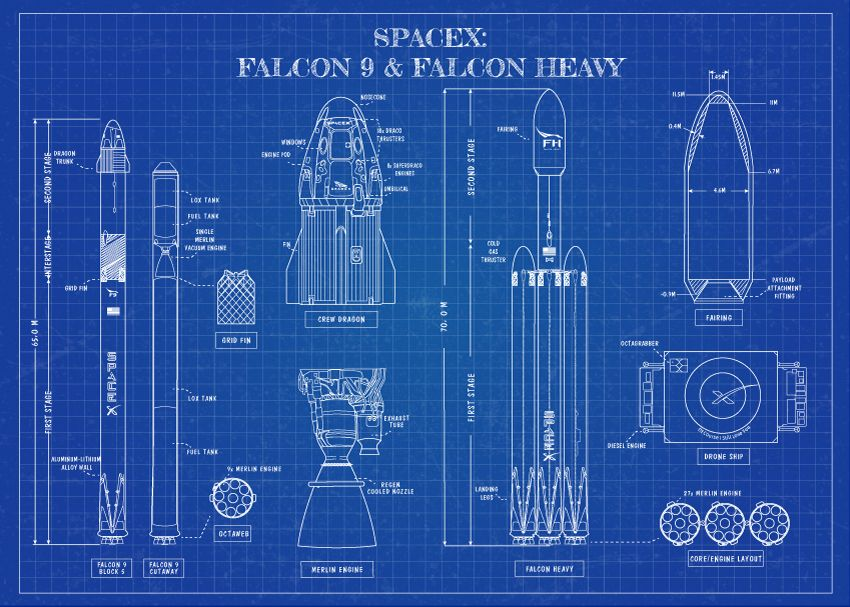
\includegraphics[scale=0.45]{gambar/blueprint.jpg}
%   % Keterangan gambar yang diinputkan
%   \caption{\emph{Blueprint} roket yang akan diuji coba \parencite{SpaceXBlueprint}}
%   % Label referensi dari gambar yang diinputkan
%   \label{fig:Blueprint}
% \end{figure}
% % Contoh penggunaan referensi dari gambar yang diinputkan
% Pada \emph{blueprint} yang tertera di Gambar \ref{fig:Blueprint}. \lipsum[12]

\section{Metode yang digunakan}

Metodologi yang digunakan pada penelitian ini terdiri dari beberapa tahapan seperti yang
ditunjukkan pada gambar berikut.

\begin{figure} [H] \centering
  % Nama dari file gambar yang diinputkan
  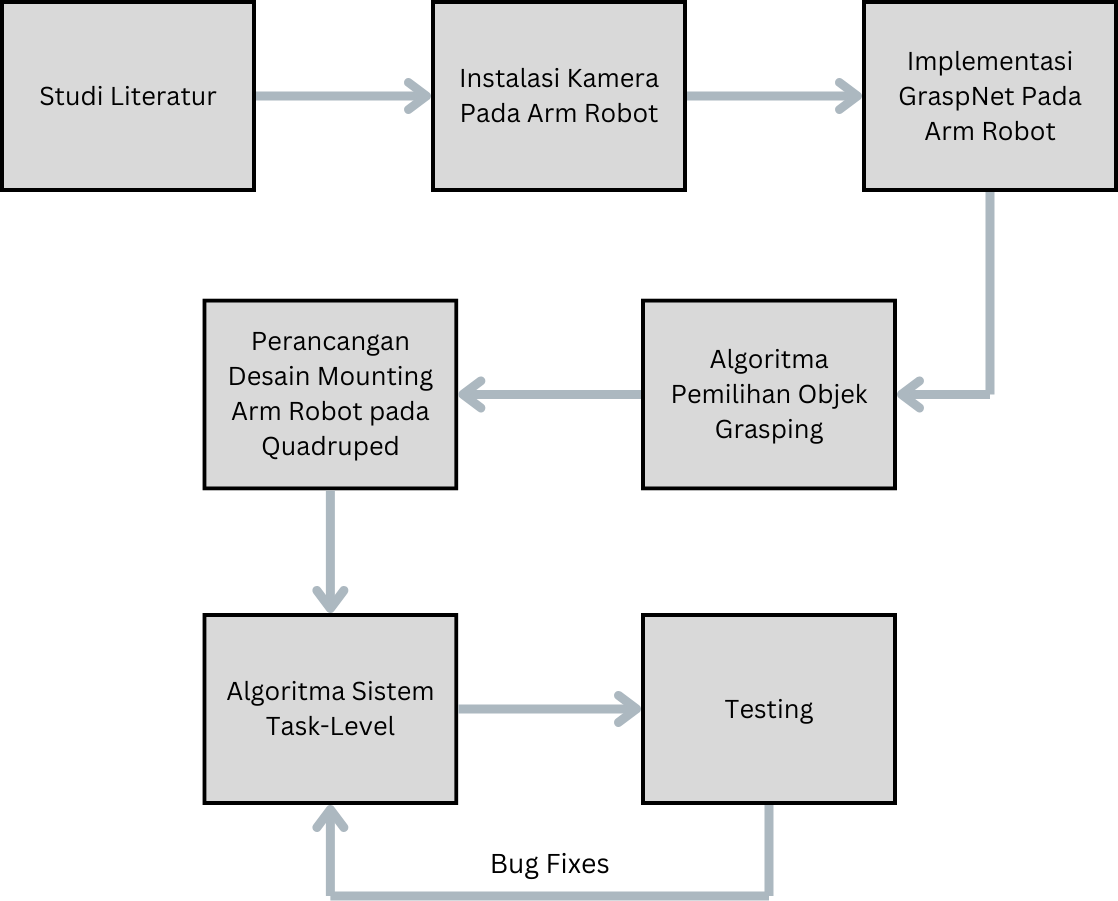
\includegraphics[scale=0.4]{gambar/Blok Diagram Metodologi.png}
  % Keterangan gambar yang diinputkan
  \caption{Blok Diagram Perancangan Penelitian}
  % Label referensi dari gambar yang diinputkan
  \label{fig:diagram_metode}
\end{figure}

Berikut merupakan penjelasan dari tiap tahapan pada metode penelitian di atas :
\begin{enumerate}
  \item \textbf{Studi Literatur} : Tahap awal dalam penelitian ini adalah melakukan studi literatur untuk memahami konsep
  dan teknologi yang mendasari penelitian. Studi literatur dilakukan terhadap berbagai sumber
  seperti jurnal ilmiah, buku referensi, dan publikasi konferensi yang membahas topik terkait,
  seperti robot lengan (\emph{robotic arm}), robot \emph{quadruped}, GraspNet, algoritma \emph{grasping}, serta
  integrasi sensor dan sistem kendali. Penelitian sebelumnya yang relevan akan dikaji untuk
  memahami pendekatan yang telah dilakukan dan menemukan potensi perbaikan atau inovasi
  yang dapat diterapkan dalam penelitian ini. Literatur terkait metode pemasangan kamera
  untuk persepsi visual pada robot lengan juga dikaji untuk memilih konfigurasi sensor yang optimal.

  \item \textbf{Instalasi Kamera Pada Robot Lengan} : Tahap ini bertujuan untuk mengintegrasikan
  sistem persepsi visual menggunakan kamera pada robot lengan. Kamera akan dipasang di posisi
  yang memungkinkan robot melihat objek yang akan diambil, yaitu di pangkal bagian \emph{gripper}.
  Posisi ini dipilih karena memungkinkan untuk robot dapat mengontrol sudut yang dilihat oleh kamera.
  Proses pemasangan menggunakan mounting yang didesain dan dicetak menggunakan \emph{3D Printer}

  \item \textbf{Implementasi GraspNet Pada Robot Lengan} : Pada tahap ini, algoritma GraspNet
  akan diimplementasikan untuk mendeteksi \emph{pose} optimal dalam proses \emph{grasping}.
  GraspNet merupakan model berbasis \emph{machine learning} yang mampu memprediksi berbagai
  kemungkinan posisi dan orientasi tangan robot dalam mencengkeram suatu objek. Model GraspNet
  akan diterapkan pada data citra yang diperoleh dari kamera, sehingga sistem dapat menentukan
  titik \emph{grasping} terbaik dengan mempertimbangkan faktor seperti bentuk, orientasi, dan jenis objek.
  Pengujian awal dilakukan untuk menilai performa algoritma dalam mendeteksi \emph{pose} \emph{grasping}
  pada berbagai jenis objek. Jika diperlukan, model GraspNet dapat disesuaikan atau
  di-\emph{fine-tune} untuk meningkatkan akurasi dan efisiensi sistem.

  \item \textbf{Algoritma Pemilihan Objek Grasping} : Pemilihan objek yang akan di-\emph{grasp} dilakukan
  oleh operator (manusia) melalui antarmuka interaktif, sehingga menghilangkan kemungkinan kesalahan
  keputusan robot dalam melakukan pemilihan objek. Bounding box akan ditampilkan pada objek yang terdeteksi
  melalui kamera, sehingga membiarkan operator memilih objek tersebut melalui klik pada GUI. Setelah operator
  memilih objek, sistem akan menjalankan GraspNet untuk menentukan titik optimal grasping dan
  mengeksekusi perintah tersebut pada robot lengan. Fitur konfirmasi dan pemberian indikator pada objek
  juga ditambahkan agar interaksi lebih intuitif.

  \item \textbf{Perancangan Desain Mounting Robot Lengan Pada Quadruped} : Salah satu tantangan utama dalam penelitian
  ini adalah integrasi robot lengan dengan platform \emph{quadruped}. Desain mounting harus mempertimbangkan faktor-faktor
  seperti keseimbangan, distribusi beban, dan fleksibilitas gerakan. Perancangan dilakukan menggunakan perangkat lunak CAD
  seperti Fusion 360 untuk memastikan desain yang optimal. Proses pemasangan dilakukan dengan memastikan bahwa robot
  \emph{quadruped} tetap dapat bergerak dengan stabil meskipun membawa robot lengan.

  \item \textbf{Algoritma Sistem Task-Level} : Setelah integrasi perangkat keras selesai, tahap selanjutnya adalah
  mengembangkan algoritma \emph{task-level} yang mengoordinasikan gerakan robot lengan dan robot \emph{quadruped}.
  Algoritma ini mengatur bagaimana robot menyelesaikan tugas-tugas seperti mendekati objek, mengambilnya, dan
  membawanya ke lokasi yang diinginkan. Sistem ini juga harus mempertimbangkan faktor lingkungan, seperti menghindari
  rintangan dan menyesuaikan pergerakan sesuai kondisi medan.

  \item \textbf{Testing - Bug Fixes - Repeat} : Setelah seluruh sistem diimplementasikan, tahap uji coba dilakukan
  untuk mengevaluasi performa keseluruhan. Pengujian mencakup berbagai aspek seperti ketepatan kamera dalam menangkap
  citra dan mendeteksi objek, akurasi prediksi GraspNet dalam menentukan posisi \emph{grasping}, efektivitas algoritma
  pemilihan objek dalam membantu operator memilih target yang sesuai, stabilitas dan keseimbangan robot quadruped setelah
  pemasangan robot lengan, serta keandalan sistem \emph{task-level} dalam menyelesaikan tugas. Jika ditemukan bug atau
  kekurangan dalam sistem, perbaikan dilakukan dengan menyesuaikan algoritma atau komponen perangkat keras yang bermasalah.
  Setelah perbaikan, pengujian diulang hingga sistem bekerja secara optimal dan memenuhi kriteria keberhasilan yang telah ditetapkan.
  
\end{enumerate}